\documentclass{beamer}
\usetheme{CambridgeUS}
\usepackage[utf8]{inputenc}
\usepackage{transparent}
\usepackage{tikz}
%=== define colors ===
\setbeamercolor{title}{fg=black}

%=== define outline ===
\AtBeginSection[]
{
  \begin{frame}<beamer>
    %\frametitle{Outline for section \thesection}
    \tableofcontents[currentsection,
    hideothersubsections, 
	sectionstyle=show/shaded,
	]
  \end{frame}
}
\makeatother
\setbeamertemplate{footline}
{
    \leavevmode%
    \hbox{%
        \begin{beamercolorbox}[wd=.3\paperwidth,ht=2.25ex,dp=1ex,center]{author in head/foot}%
            \usebeamerfont{author in head/foot}\insertshortauthor
        \end{beamercolorbox}%
        \begin{beamercolorbox}[wd=.4\paperwidth,ht=2.25ex,dp=1ex,center]{title in head/foot}%
            \usebeamerfont{title in head/foot}\insertshorttitle
        \end{beamercolorbox}%
        \begin{beamercolorbox}[wd=.3\paperwidth,ht=2.25ex,dp=1ex,center]{date in head/foot}%
            \today\  [\insertframenumber{} / \inserttotalframenumber]\hspace*{1ex}
        \end{beamercolorbox}}%
    \vskip0pt%
}
\makeatletter

\title{Clock Pendulum Analyzer - PAWI Projekt}
\author{Tobias Kreienbühl \& Daniel Föhn}
\institute{Hochschule Luzern, Informatik}
\date{\today}
 

\begin{document}
\begin{frame}
	\titlepage
\end{frame}

\section{Überblick}
\begin{frame}

\end{frame}

\section{Hardware Board}
\begin{frame}

\end{frame}

%!TEX root=ClockPendulumAnalyzer.tex
\section{Raspberry Pi}
\begin{frame}
%image with all the technologies
\end{frame}

\subsection{Aufbau - Architektur}
\begin{frame}
    \frametitle{Aufbau - Architektur}
    \begin{columns}[c] % the "c" option specifies center vertical alignment
        \column{.5\textwidth}
        \begin{itemize}
            \item<1->3-Layer Architektur
            \item<1->mögliche 2-Tier Verteilung
            \item<1->Daten-Transfer-Objekt und REST
        \end{itemize}
        \column{.5\textwidth} % column designated by a command
        \begin{figure}
            \centering
            \begin{overprint}
                \onslide<1>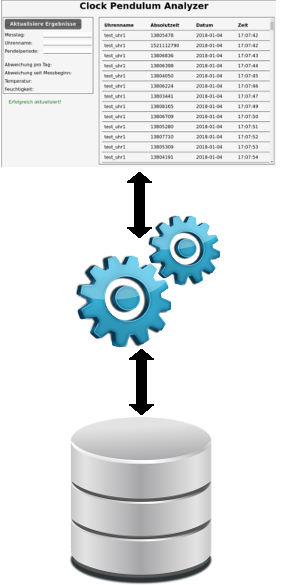
\includegraphics[width=.5\textwidth]{3layer.png}
                \onslide<2->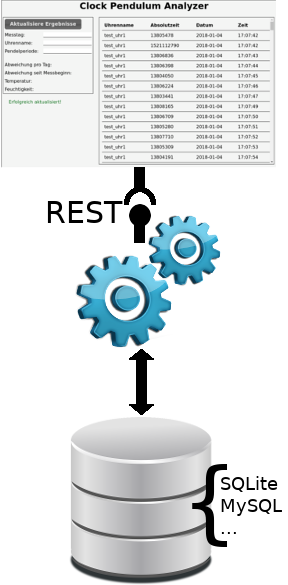
\includegraphics[width=.5\textwidth]{3layer_rest.png}
            \end{overprint}
        \end{figure}
    \end{columns}
\end{frame}

\subsection{Technologien}
\begin{frame}

\end{frame}

\subsection{C++ Software}
\begin{frame}

\end{frame}

\subsection{Schnittstellen}
\begin{frame}

\end{frame}

\section{Schwierigkeiten}
\begin{frame}
    \frametitle{Aufgetretene Probleme}
	\begin{itemize}
        \item<1-> Schwierigkeiten bei $I^2C$ auf ArchLinux ARM
        \item<1-> REST-TCP Socket auf C++
        \item<1-> sowie CORS (Cross-Origin Resource Sharing)
        \item<2->
    \end{itemize}
\end{frame}

\section{Ausblick}
\begin{frame}
	\frametitle{Ausblick}
	\begin{itemize}
		\item Aufwertung der Genauigkeit durch hochgenauen Oszillator
		\item Reduktion der Interrupt-Zeiten durch schnelleren Controller
		\item Verwenden eines genaueren Sensors
        \item Erweiterung / Realisierung einer Benutzeroberfläche
	\end{itemize}
\end{frame}

\section{Quellen}
\begin{frame}
%https://cdn.pixabay.com/photo/2014/04/03/10/08/database-309919_960_720.png
%https://www.kinvey.com/wp-content/uploads/2014/04/data.png
%https://vignette.wikia.nocookie.net/verse-and-dimensions/images/9/9f/Double_arrow_symbol_-_red.svg.png/revision/latest?cb=20170327191524
\end{frame}

\end{document}